%%%%%%%%%%%%%%%%%%%%%%%%%%%%%%%%%%%%%%%%%%%%%%%%%%%%%%%%%%%%%%%%%%%%%%%%%%%%%%%%%%%%%%%%%%%%%%%%%%%%%%%%%%
\newpage
\appendix 

\section{Properties of Embedding based Value Functions}
\label{app:prop_emb}

\begin{proposition}\label{prop:v_logvol}
The log-volume value function $v_{\text{logvol}}$ satisfies the following properties:
\begin{enumerate}
    \item \textbf{Monotonicity and Non-Negativity:} $v_{\text{logvol}}(S') \ge 0$ for all $S' \subseteq [n]$, and $v_{\text{logvol}}$ is strictly monotone: $S' \subseteq T' \implies v_{\text{logvol}}(S') \le v_{\text{logvol}}(T')$.
    \item \textbf{Exact Marginal Gain:} For any $i \notin S'$, let $\mathbf{r}_{\perp} := (\mathbf{I}_d - \mathbf{P}_{\{S'\}})\mathbf{r}$ and $\mathbf{m}_{i, \perp} := (\mathbf{I}_d - \mathbf{P}_{\{S'\}})\mathbf{m}_i$ be the residual vectors orthogonal to $\mathcal{U}_{\{S'\}}$. If $\mathbf{m}_{i, \perp} \neq \mathbf{0}$, the marginal gain evaluates in closed form to:
    \begin{align}\label{eq:marginal_logvol}
        \Delta v_{\text{logvol}}(S', i) = -\frac{1}{2} \log\big(1 - \cos^2 \theta_i(S')\big) \ge 0, \qquad \text{where } \cos \theta_i(S') := \frac{\langle \mathbf{r}_{\perp}, \mathbf{m}_{i, \perp} \rangle}{\|\mathbf{r}_{\perp}\|_2 \|\mathbf{m}_{i, \perp}\|_2},
    \end{align}
    and $\Delta v_{\text{logvol}}(S', i) := 0$ if $\mathbf{m}_{i, \perp} = \mathbf{0}$.
    \item \textbf{Guaranteed Non-Negative Shapley Allocations:} Every snippet receives a non-negative raw Shapley value: $\phi_i(v_{\text{logvol}}) \ge 0$ for all $i \in [n]$, with $\sum_{i=1}^n \phi_i(v_{\text{logvol}}) = -\log d_{\perp}(\mathbf{r}, \mathcal{U}_{\{[n]\}})$.
\end{enumerate}
\end{proposition}

\begin{proof}
(1) Because $\|\mathbf{r}\|_2 = 1$, the orthogonal distance satisfies $d_{\perp}(\mathbf{r}, \mathcal{U}_{\{S'\}}) \in [0, 1]$, which implies $-\log d_{\perp} \ge 0$. Adding vectors expands the subspace ($\mathcal{U}_{\{S'\}} \subseteq \mathcal{U}_{\{T'\}}$), which monotonically non-increases the residual distance, rendering $v_{\text{logvol}}$ monotone. 
(2) Since $\mathcal{U}_{\{S' \cup \{i\}\}} = \mathcal{U}_{\{S'\}} \oplus \operatorname{span}(\mathbf{m}_{i, \perp})$, projecting $\mathbf{r}_{\perp}$ onto the unit vector $\mathbf{u} = \mathbf{m}_{i, \perp} / \|\mathbf{m}_{i, \perp}\|_2$ yields:
\begin{align*}
    d_{\perp}^2(\mathbf{r}, \mathcal{U}_{\{S' \cup \{i\}\}}) = \|\mathbf{r}_{\perp}\|_2^2 - \langle \mathbf{r}_{\perp}, \mathbf{u} \rangle^2 = \|\mathbf{r}_{\perp}\|_2^2 \big(1 - \cos^2 \theta_i(S')\big).
\end{align*}
Taking $-\frac{1}{2}\log$ of the ratio $d_{\perp}^2(\mathbf{r}, \mathcal{U}_{\{S' \cup \{i\}\}}) / d_{\perp}^2(\mathbf{r}, \mathcal{U}_{\{S'\}})$ yields Equation~\eqref{eq:marginal_logvol}. By the Cauchy--Schwarz inequality, $\cos^2 \theta_i(S') \in [0, 1]$, ensuring the argument of the logarithm is in $(0, 1]$, so $\Delta v_{\text{logvol}} \ge 0$. 
(3) Follows directly because the Shapley value is a convex combination of non-negative marginal gains.
\end{proof}


\begin{proposition}[Spectral Mutual Information Interpretation]\label{prop:v_ent}
Let $\boldsymbol{\rho} := \boldsymbol{\rho}(\mathbf{G}^{+}_{\{S'\}})$ and $\boldsymbol{\sigma} := \boldsymbol{\rho}(\bar{\mathbf{G}}^{+}_{\{S'\}})$. Then:
\begin{enumerate}
    \item $v_{\text{ent}}(S') = D(\boldsymbol{\rho} \,\|\, \boldsymbol{\sigma}) := \operatorname{Tr}\big(\boldsymbol{\rho}(\log \boldsymbol{\rho} - \log \boldsymbol{\sigma})\big)$, where $D(\cdot \,\|\, \cdot)$ is the quantum relative entropy.
    \item $v_{\text{ent}}(S') \ge 0$, with $v_{\text{ent}}(S') = 0$ if and only if $\mathbf{M}_{\{S'\}}^\top \mathbf{r} = \mathbf{0}$ ($\mathbf{r} \perp \mathcal{U}_{\{S'\}}$).
    \item $v_{\text{ent}}(S') \le \log 2$ for all coalitions, ensuring $v_{\text{ent}}$ is universally bounded without regularization.
\end{enumerate}
\end{proposition}

\begin{proof}
(1) Since $\boldsymbol{\sigma}$ is block-diagonal, $\log \boldsymbol{\sigma}$ is also block-diagonal on its support. Because the diagonal blocks of $\boldsymbol{\rho}$ and $\boldsymbol{\sigma}$ are identical, $\operatorname{Tr}(\boldsymbol{\rho} \log \boldsymbol{\sigma}) = \operatorname{Tr}(\boldsymbol{\sigma} \log \boldsymbol{\sigma}) = -\mathcal{H}(\bar{\mathbf{G}}^{+}_{\{S'\}})$, establishing $v_{\text{ent}}(S') = D(\boldsymbol{\rho} \,\|\, \boldsymbol{\sigma})$. 
(2) By Klein's inequality, $D(\boldsymbol{\rho} \,\|\, \boldsymbol{\sigma}) \ge 0$, with equality holding if and only if $\boldsymbol{\rho} = \boldsymbol{\sigma}$, which occurs precisely when the cross-term $\mathbf{g}_{\{S'\}} = \mathbf{M}_{\{S'\}}^\top \mathbf{r} = \mathbf{0}$. 
(3) Noting that $\boldsymbol{\sigma} = \frac{1}{2}(\boldsymbol{\rho} + \mathbf{U}\boldsymbol{\rho}\mathbf{U}^\top)$ for the unitary matrix $\mathbf{U} = \operatorname{diag}(\mathbf{I}_k, -1)$, subadditivity of entropy bounds the entropy increase by $\mathcal{H}(\boldsymbol{\sigma}) - \mathcal{H}(\boldsymbol{\rho}) \le \log 2$.
\end{proof}

\section{Tractable Approximation of Shapley value via Permutation Sampling}
\label{subsec:tractable_approximation}

To overcome the exponential $\mathcal{O}(2^n)$ bottleneck of the exact Shapley formulation, one can approximate the attribution vector using Monte Carlo sampling over permutations. This approach is widely considered part of the literature's folklore. The permutation-based Monte Carlo approximation of the Shapley value was first introduced in cooperative game theory by Mann and Shapley~\cite{mann1960values}.  We formalize this unbiased estimator and provide its proof below.

\begin{lemma}\label{lemma:unbiased_estimator}
\textbf{(Unbiased Estimator of the Shapley Vector).}
Let $\boldsymbol{\Phi}(v) = (\phi_1(v), \dots, \phi_n(v))^\top \in \mathbb{R}^n$ be the exact Shapley attribution vector under any valid characteristic function $v$ with $v(\emptyset) = 0$. Let $\Pi([n])$ denote the symmetric group of all $n!$ permutations of the index set $[n]$. For a permutation $\pi \in \Pi([n])$ sampled uniformly at random, let $S_i^\pi := \{j \in [n] \mid \pi(j) < \pi(i)\}$ denote the subset of players preceding player $i$ in $\pi$. Define the stochastic marginal gain vector $\mathbf{m}^\pi := (m_1^\pi, \dots, m_n^\pi)^\top \in \mathbb{R}^n$ where $m_i^\pi := \Delta v(S_i^\pi, i)$. Then $\mathbf{m}^\pi$ is an unbiased estimator of the true Shapley vector:
\begin{align}
    \mathbb{E}_{\pi \sim \Pi([n])}[\mathbf{m}^\pi] = \boldsymbol{\Phi}(v).
\end{align}
\end{lemma}

By generating a small set of $K \ll n!$ uniform random permutations, the true Shapley vector can be approximated in strictly polynomial time $\mathcal{O}(K \cdot n \cdot \mathcal{C})$, where $\mathcal{C}$ is the evaluation cost of the characteristic function.  While evaluating even a small number of paths is prohibitively expensive when using autoregressive forward passes ($C = \mathcal{C}_{\text{LLM}}$), this approximation becomes extremely practical under our proposed embedding-based geometric frameworks where $\mathcal{C} = \mathcal{O}(d^2)$, see in Section \ref{}.


\begin{proofof}{Lemma~\ref{lemma:unbiased_estimator}}
To show that the expectation holds, we evaluate the expectation of an arbitrary $i$-th component, $\mathbb{E}_\pi[m_i^\pi]$. Since the permutation $\pi$ is sampled uniformly from $\Pi([n])$, each permutation occurs with probability $1/n!$. The expected value of the marginal gain of snippet $i$ is:
\begin{align}
    \mathbb{E}_{\pi}[m_i^\pi] = \sum_{\pi \in \Pi([n])} \frac{1}{n!} \Delta v(S_i^\pi, i).
\end{align}
We partition the summation over all permutations by grouping them according to the unique unordered subset of preceding elements. For a fixed subset $S' \subseteq [n] \setminus \{i\}$ of size $k = |S'|$, we count the number of permutations $\pi \in \Pi([n])$ that satisfy $S_i^\pi = S'$. For snippet $i$ to be preceded by precisely the elements in $S'$:
\begin{enumerate}
    \item The $k$ elements within $S'$ can be arranged in the first $k$ positions of the permutation in $k!$ different ways.
    \item The element $i$ must be fixed at position $k + 1$.
    \item The remaining $(n - k - 1)$ elements in $[n] \setminus (S' \cup \{i\})$ can be arranged in the remaining positions in $(n - k - 1)!$ different ways.
\end{enumerate}
Thus, there are exactly $|S'|!(n - |S'| - 1)!$ permutations that yield the exact marginal context subset $S_i^\pi = S'$. Replacing the sum over permutations with a sum over all possible subsets $S' \subseteq [n] \setminus \{i\}$ weighted by this combinatorial factor yields:
\begin{align}
    \mathbb{E}_{\pi}[m_i^\pi] = \sum_{S' \subseteq [n] \setminus \{i\}} \frac{|S'|!(n - |S'| - 1)!}{n!} \Delta v(S', i).
\end{align}
This formulation is exactly the canonical subset-based definition of the exact Shapley value $\phi_i(v)$. Since $\mathbb{E}_{\pi}[m_i^\pi] = \phi_i(v)$ holds for every element $i \in [n]$, it follows that the joint vector expectation exactly recovers the full attribution vector $\mathbb{E}_\pi[\mathbf{m}^\pi] = \boldsymbol{\Phi}(v)$, completing the proof.
\end{proofof}

%%%%%%%%%%%%%%%%%%%%%%%%%%%%%%%%%%%%%%%%%%%%%%%%%%%%%%%%%%%%%%%%%%%%%%%%%%%%%%%%%%%%%%%%%%%%%%%%%%%%%%%%%%%%

\section{Covariance Structure and Bernstein Concentration}
\label{app:bernstein_concentration}

Let $\pi_1, \dots, \pi_K \overset{\text{i.i.d.}}{\sim} \Pi([n])$ be $K$ permutations sampled uniformly at random. For each trajectory $\pi_k$, the stochastic marginal gain vector is $\mathbf{m}^{\pi_k} = (m_1^{\pi_k}, \dots, m_n^{\pi_k})^\top \in \mathbb{R}^n$, where $m_i^{\pi_k} := \Delta v(S_i^{\pi_k}, i)$. The empirical Monte Carlo Shapley estimator is:
\begin{align}
    \bar{\mathbf{m}}_K := \frac{1}{K} \sum_{k=1}^K \mathbf{m}^{\pi_k}, \qquad \text{with } \mathbb{E}[\bar{\mathbf{m}}_K] = \boldsymbol{\Phi}(v).
\end{align}

\paragraph{Telescoping Sum and Covariance Identity.}
Along any permutation $\pi$, the marginal contributions telescope across the entire grand coalition:
\begin{align}\label{eq:telescoping_sum}
    \sum_{i=1}^n m_i^\pi = \sum_{k=1}^n \Big( v(\{\pi_1, \dots, \pi_k\}) - v(\{\pi_1, \dots, \pi_{k-1}\}) \Big) = v([n]) - v(\emptyset) = v([n]).
\end{align}
Because the sum is a deterministic constant, $\operatorname{Var}\big(\sum_{i=1}^n m_i^\pi\big) = 0$. Expanding the variance of the sum yields the zero-sum cross-covariance identity:
\begin{align}\label{eq:zero_sum_cov}
    \sum_{j=1}^n \operatorname{Cov}(m_i^\pi, m_j^\pi) = 0 \quad \Longleftrightarrow \quad \sum_{j \neq i} \operatorname{Cov}(m_i^\pi, m_j^\pi) = -\sigma_i^2,
\end{align}
where $\sigma_i^2 := \operatorname{Var}(m_i^\pi) = \mathbb{E}[(m_i^\pi - \phi_i(v))^2]$. The negative total covariance demonstrates that individual coordinates compete directly for semantic volume along any single trajectory.

\paragraph{Bernstein Concentration Bound.}
Assume that the marginal contributions are bounded such that $\sup_{S', i} |\Delta v(S', i)| \le B$. Then for each player $i \in [n]$, the centered variable $X_k := m_i^{\pi_k} - \phi_i(v)$ satisfies $\mathbb{E}[X_k] = 0$, $\mathbb{E}[X_k^2] = \sigma_i^2$, and $|X_k| \le 2B$ almost surely.

\begin{theorem}\label{thm:bernstein_shapley}
Let $\sigma_{\max}^2 := \max_{i \in [n]} \sigma_i^2$. For any error tolerance $\epsilon > 0$, the empirical estimator $\bar{\mathbf{m}}_K$ concentrates around the exact Shapley vector $\boldsymbol{\Phi}(v)$ as:
\begin{align}
    \mathbb{P}\Big( \|\bar{\mathbf{m}}_K - \boldsymbol{\Phi}(v)\|_\infty \ge \epsilon \Big) \le 2n \exp\left( -\frac{K \epsilon^2}{2 \sigma_{\max}^2 + \frac{4}{3} B \epsilon} \right).
\end{align}
Consequently, to guarantee that $\|\bar{\mathbf{m}}_K - \boldsymbol{\Phi}(v)\|_\infty \le \epsilon$ with probability at least $1 - \delta$, it suffices to sample:
\begin{align}
    K \ge \left( \frac{2 \sigma_{\max}^2}{\epsilon^2} + \frac{4 B}{3 \epsilon} \right) \log\left( \frac{2n}{\delta} \right) = \mathcal{O}\left( \frac{\sigma_{\max}^2}{\epsilon^2} \log\left(\frac{n}{\delta}\right) \right)
\end{align}
permutations.
\end{theorem}

\begin{proof}
Applying Bernstein's inequality to the sum of $K$ independent, zero-mean, bounded random variables $\sum_{k=1}^K (m_i^{\pi_k} - \phi_i(v))$ yields:
\begin{align}
    \mathbb{P}\Big( |\bar{m}_{K, i} - \phi_i(v)| \ge \epsilon \Big) = \mathbb{P}\left( \left|\sum_{k=1}^K X_k\right| \ge K \epsilon \right) \le 2 \exp\left( -\frac{K^2 \epsilon^2}{2 K \sigma_i^2 + \frac{2}{3}(2B)(K \epsilon)} \right) = 2 \exp\left( -\frac{K \epsilon^2}{2 \sigma_i^2 + \frac{4}{3} B \epsilon} \right).
\end{align}
Applying the union bound over all $n$ coordinates immediately gives the $\ell_\infty$ bound. Setting the error probability equal to $\delta$ and solving for $K$ yields the sample complexity bound.
\end{proof}



%%%%%%%%%%%%%%%%%%%%%%%%%%%%%%%%%%%%%%%%%%%%%%%%%%%%%%%%%%%%%%%%%%%%%%%%%%%%%%%%%%%%%%%%%%%%%%%%%%%%%%%%%%%%
% Appendix material (place after \appendix).
%%%%%%%%%%%%%%%%%%%%%%%%%%%%%%%%%%%%%%%%%%%%%%%%%%%%%%%%%%%%%%%%%%%%%%%%%%%%%%%%%%%%%%%%%%%%%%%%%%%%%%%%%%%%
\section{Additional Experimental Results}
\label{app:exp_correct}

The supporting-fact labels of HotpotQA describe the evidence for the \emph{correct} answer. Table~\ref{tab:exp_correct} repeats Tables~\ref{tab:exp_main} and~\ref{tab:exp_values} on the $160$ instances ($80\%$) in which the generated response contains the normalized gold answer. All differences lie well within the confidence intervals. The exact likelihood reference places $95.7\%$ of the credit on the supporting facts (AUROC $0.92$, P@2 $86.6\%$); EATT with $v_{\text{logvol}}$ reaches $92.8\%$ mass and AUROC $0.91$; GATT-TCR with $v_{\text{logvol}}$ reaches $r = 0.79$ and $79.9\%$ mass; VATT with $v_{\text{proj}}$ reaches $r = 0.91$, $92.4\%$ mass, AUROC $0.93$ and P@2 $88.4\%$; and the mean global context weight remains $w = 0.95$.

\begin{table}[t]
\centering
\small
\setlength{\tabcolsep}{2.6pt}
\resizebox{\linewidth}{!}{%
\begin{tabular}{lllcccccccccc}
\toprule
 & & & & \multicolumn{5}{c}{Agreement with Exact LLH-Shapley} & \multicolumn{3}{c}{Supporting facts} \\
\cmidrule(lr){5-9} \cmidrule(lr){10-12}
Method & $v$ & Link & Passes & Pearson $r$ & Spearman $\rho$ & Kendall $\tau$ & MAE (pp) $\downarrow$ & Top-1 (\%) & Mass (\%) & AUROC & P@2 (\%) \\
\midrule
\multicolumn{12}{l}{\emph{Proposed geometric methods (two LLM passes)}} \\
EATT (Gecko) & $v_{\mathrm{vol}}$ & floor & $2^\dagger$ & 0.73{\scriptsize$\pm$0.06} & 0.62{\scriptsize$\pm$0.05} & 0.54{\scriptsize$\pm$0.04} & 10.9{\scriptsize$\pm$1.3} & 69.4{\scriptsize$\pm$7.2} & 89.5{\scriptsize$\pm$2.5} & 0.88{\scriptsize$\pm$0.03} & 78.4{\scriptsize$\pm$3.8} \\
EATT (Gecko) & $v_{\mathrm{logvol}}$ & floor & $2^\dagger$ & 0.74{\scriptsize$\pm$0.05} & 0.69{\scriptsize$\pm$0.04} & 0.60{\scriptsize$\pm$0.03} & 10.7{\scriptsize$\pm$1.4} & 69.4{\scriptsize$\pm$7.2} & \textbf{92.8}{\scriptsize$\pm$2.1} & 0.91{\scriptsize$\pm$0.02} & 84.1{\scriptsize$\pm$3.6} \\
EATT (Gecko) & $v_{\mathrm{ent}}$ & floor & $2^\dagger$ & 0.73{\scriptsize$\pm$0.05} & 0.66{\scriptsize$\pm$0.04} & 0.58{\scriptsize$\pm$0.04} & 11.0{\scriptsize$\pm$1.3} & 65.6{\scriptsize$\pm$7.5} & 86.7{\scriptsize$\pm$2.6} & 0.89{\scriptsize$\pm$0.03} & 79.7{\scriptsize$\pm$3.8} \\
\addlinespace[2pt]
GATT-RCB & $v_{\mathrm{vol}}$ & floor & 2.0 & 0.70{\scriptsize$\pm$0.06} & 0.58{\scriptsize$\pm$0.05} & 0.50{\scriptsize$\pm$0.05} & 12.5{\scriptsize$\pm$1.6} & 64.4{\scriptsize$\pm$7.5} & 74.5{\scriptsize$\pm$3.4} & 0.82{\scriptsize$\pm$0.03} & 70.6{\scriptsize$\pm$4.7} \\
GATT-RCB & $v_{\mathrm{logvol}}$ & floor & 2.0 & 0.72{\scriptsize$\pm$0.06} & 0.61{\scriptsize$\pm$0.05} & 0.53{\scriptsize$\pm$0.04} & 11.9{\scriptsize$\pm$1.5} & 66.2{\scriptsize$\pm$7.5} & 76.1{\scriptsize$\pm$3.3} & 0.83{\scriptsize$\pm$0.03} & 72.5{\scriptsize$\pm$4.4} \\
GATT-RCB & $v_{\mathrm{ent}}$ & floor & 2.0 & 0.74{\scriptsize$\pm$0.05} & 0.62{\scriptsize$\pm$0.04} & 0.54{\scriptsize$\pm$0.04} & 12.0{\scriptsize$\pm$1.5} & 66.9{\scriptsize$\pm$7.2} & 73.3{\scriptsize$\pm$3.3} & 0.84{\scriptsize$\pm$0.03} & 71.2{\scriptsize$\pm$4.4} \\
\addlinespace[2pt]
GATT-TCR & $v_{\mathrm{vol}}$ & floor & 2.0 & 0.28{\scriptsize$\pm$0.07} & 0.35{\scriptsize$\pm$0.05} & 0.30{\scriptsize$\pm$0.04} & 20.5{\scriptsize$\pm$1.5} & 23.8{\scriptsize$\pm$6.6} & 46.7{\scriptsize$\pm$4.3} & 0.68{\scriptsize$\pm$0.03} & 52.8{\scriptsize$\pm$3.4} \\
GATT-TCR & $v_{\mathrm{logvol}}$ & floor & 2.0 & 0.79{\scriptsize$\pm$0.05} & 0.64{\scriptsize$\pm$0.04} & 0.56{\scriptsize$\pm$0.04} & 10.0{\scriptsize$\pm$1.4} & 76.2{\scriptsize$\pm$6.6} & 79.9{\scriptsize$\pm$3.2} & 0.84{\scriptsize$\pm$0.03} & 70.6{\scriptsize$\pm$4.1} \\
GATT-TCR & $v_{\mathrm{ent}}$ & floor & 2.0 & 0.31{\scriptsize$\pm$0.07} & 0.36{\scriptsize$\pm$0.05} & 0.31{\scriptsize$\pm$0.04} & 20.2{\scriptsize$\pm$1.5} & 26.9{\scriptsize$\pm$6.6} & 46.2{\scriptsize$\pm$4.2} & 0.67{\scriptsize$\pm$0.03} & 51.2{\scriptsize$\pm$4.1} \\
\addlinespace[2pt]
VATT & $v_{\mathrm{proj}}$ & floor & 2.0 & \textbf{0.91}{\scriptsize$\pm$0.03} & 0.79{\scriptsize$\pm$0.02} & 0.70{\scriptsize$\pm$0.02} & \textbf{5.8}{\scriptsize$\pm$0.8} & \textbf{81.9}{\scriptsize$\pm$5.9} & 92.4{\scriptsize$\pm$2.1} & \textbf{0.93}{\scriptsize$\pm$0.02} & \textbf{88.4}{\scriptsize$\pm$3.3} \\
VATT & $v_{\mathrm{logvol}}$ & floor & 2.0 & 0.90{\scriptsize$\pm$0.03} & 0.77{\scriptsize$\pm$0.02} & 0.68{\scriptsize$\pm$0.02} & 6.3{\scriptsize$\pm$0.8} & 79.4{\scriptsize$\pm$6.2} & 90.3{\scriptsize$\pm$2.2} & 0.92{\scriptsize$\pm$0.02} & 85.9{\scriptsize$\pm$3.6} \\
VATT & $v_{\mathrm{vol}}$ & rect. & 2.0 & 0.89{\scriptsize$\pm$0.03} & \textbf{0.86}{\scriptsize$\pm$0.03} & \textbf{0.81}{\scriptsize$\pm$0.03} & 6.8{\scriptsize$\pm$0.9} & 77.5{\scriptsize$\pm$6.6} & 91.9{\scriptsize$\pm$2.6} & 0.92{\scriptsize$\pm$0.02} & 86.2{\scriptsize$\pm$3.6} \\
VATT & $v_{\mathrm{ent}}$ & floor & 2.0 & 0.89{\scriptsize$\pm$0.03} & 0.76{\scriptsize$\pm$0.02} & 0.67{\scriptsize$\pm$0.02} & 7.1{\scriptsize$\pm$0.8} & 78.1{\scriptsize$\pm$6.2} & 87.1{\scriptsize$\pm$2.4} & 0.91{\scriptsize$\pm$0.03} & 84.4{\scriptsize$\pm$3.7} \\
\midrule
\multicolumn{12}{l}{\emph{Gradient and subset-ablation baselines}} \\
Gradient $\times$ Input & $\nabla F$ & rect. & $2.0^\ddagger$ & 0.00{\scriptsize$\pm$0.07} & 0.02{\scriptsize$\pm$0.07} & 0.01{\scriptsize$\pm$0.06} & 25.8{\scriptsize$\pm$1.6} & 19.4{\scriptsize$\pm$6.2} & 31.8{\scriptsize$\pm$4.9} & 0.49{\scriptsize$\pm$0.04} & 30.6{\scriptsize$\pm$4.5} \\
Integrated Gradients (16) & $\nabla F$ & rect. & $17.0^\ddagger$ & 0.04{\scriptsize$\pm$0.07} & 0.08{\scriptsize$\pm$0.07} & 0.07{\scriptsize$\pm$0.06} & 24.6{\scriptsize$\pm$1.2} & 16.2{\scriptsize$\pm$5.6} & 36.0{\scriptsize$\pm$4.9} & 0.53{\scriptsize$\pm$0.04} & 34.7{\scriptsize$\pm$4.7} \\
LOO & $v_{\mathrm{LL}}$ & rect. & 8.0 & 0.97{\scriptsize$\pm$0.02} & 0.78{\scriptsize$\pm$0.03} & 0.72{\scriptsize$\pm$0.03} & 3.4{\scriptsize$\pm$0.6} & 95.0{\scriptsize$\pm$3.4} & 93.8{\scriptsize$\pm$2.7} & 0.92{\scriptsize$\pm$0.02} & 87.5{\scriptsize$\pm$3.8} \\
KernelSHAP (32) & $v_{\mathrm{LL}}$ & rect. & 23.3 & 0.90{\scriptsize$\pm$0.03} & 0.79{\scriptsize$\pm$0.03} & 0.74{\scriptsize$\pm$0.03} & 6.0{\scriptsize$\pm$0.8} & 81.9{\scriptsize$\pm$5.9} & 85.2{\scriptsize$\pm$2.6} & 0.87{\scriptsize$\pm$0.03} & 76.9{\scriptsize$\pm$4.1} \\
ContextCite (32) & $v_{\mathrm{LL}}$ & rect. & 25.1 & 0.99{\scriptsize$\pm$0.01} & 0.91{\scriptsize$\pm$0.02} & 0.87{\scriptsize$\pm$0.02} & 2.6{\scriptsize$\pm$0.4} & 93.1{\scriptsize$\pm$4.1} & 92.7{\scriptsize$\pm$2.3} & 0.92{\scriptsize$\pm$0.02} & 86.9{\scriptsize$\pm$3.6} \\
LLH-Perm ($K=10$) & $v_{\mathrm{LL}}$ & rect. & 34.9 & 0.97{\scriptsize$\pm$0.01} & 0.90{\scriptsize$\pm$0.02} & 0.86{\scriptsize$\pm$0.03} & 2.7{\scriptsize$\pm$0.4} & 86.2{\scriptsize$\pm$5.3} & 94.4{\scriptsize$\pm$2.4} & 0.90{\scriptsize$\pm$0.02} & 84.1{\scriptsize$\pm$3.9} \\
\midrule
Exact LLH-Shapley (ref.) & $v_{\mathrm{LL}}$ & rect. & 63.7 & 1 & 1 & 1 & 0 & 100 & 95.7 & 0.92 & 86.6 \\
Uniform & -- & -- & 0 & -- & -- & -- & 23.7 & 10.0 & 33.8 & 0.50 & 19.4 \\
\bottomrule
\end{tabular}%
}
\caption{As Tables~\ref{tab:exp_main} and~\ref{tab:exp_values}, restricted to the $160$ instances in which the generated response contains the gold answer. Best entry among the proposed methods is in bold.}
\label{tab:exp_correct}
\end{table}


\paragraph{Citation and Easton V2.1 on answer-correct instances.}
Table~\ref{tab:exp_citation_easton_correct} repeats the separate evaluation of Section~\ref{subsec:exp_citation_easton} on the $160$ answer-correct instances. Every pattern from Table~\ref{tab:exp_citation_easton}---including prefix saturation by $m = 5$--$7$ global layers and the single-layer peak at $\ell = 29$ (\texttt{single5})---holds within roughly one percentage point: on \texttt{mean10}, Citation ($K_{\text{in}} = 3$) reaches AUROC $0.92$ and P@2 $86.6\%$ (with $g^{\text{fl},2}$ cutting MAE from $13.2$ to $5.9$\,pp and lifting supporting-fact mass from $64.8\%$ to $91.7\%$, and \texttt{mean7} reaching $5.5$\,pp MAE and $93.9\%$ mass), while Easton V2.1 (\texttt{top-2}) reaches $r = 0.92$, $\rho = 0.79$, MAE $6.4$\,pp, and $89.0\%$ mass under simplex normalization ($6.0$\,pp MAE and $89.8\%$ mass at \texttt{mean7}; $95.5\%$ mass and $5.9$\,pp MAE under $g^{\text{fl},2}$).

\begin{table}[t]
\centering
\small
\setlength{\tabcolsep}{2.8pt}
\resizebox{\linewidth}{!}{%
\begin{tabular}{lllcccccccc}
\toprule
 & & & \multicolumn{5}{c}{Agreement with Exact LLH-Shapley} & \multicolumn{3}{c}{Supporting facts} \\
\cmidrule(lr){4-8} \cmidrule(lr){9-11}
Heuristic & Red. & Link & Pearson $r$ & Spearman $\rho$ & Kendall $\tau$ & MAE (pp) $\downarrow$ & Top-1 (\%) & Mass (\%) & AUROC & P@2 (\%) \\
\midrule
\multicolumn{11}{l}{\emph{Simplex normalization (rectified link, $s_i / \sum_j s_j$, all $10$ global layers)}} \\
Citation ($K_{\mathrm{in}}{=}3, K_{\mathrm{out}}{=}10$) & \texttt{mean10} & rect. & 0.91{\scriptsize$\pm$0.02} & 0.77{\scriptsize$\pm$0.02} & 0.68{\scriptsize$\pm$0.02} & 13.2{\scriptsize$\pm$0.7} & 80.0{\scriptsize$\pm$5.9} & 64.8{\scriptsize$\pm$1.7} & 0.92{\scriptsize$\pm$0.02} & 86.6{\scriptsize$\pm$3.6} \\
Citation ($K_{\mathrm{in}}{=}1, K_{\mathrm{out}}{=}10$) & \texttt{mean10} & rect. & 0.91{\scriptsize$\pm$0.02} & 0.77{\scriptsize$\pm$0.02} & 0.68{\scriptsize$\pm$0.02} & 13.2{\scriptsize$\pm$0.7} & 80.6{\scriptsize$\pm$5.9} & 64.7{\scriptsize$\pm$1.7} & 0.92{\scriptsize$\pm$0.02} & 86.9{\scriptsize$\pm$3.6} \\
Citation ($K_{\mathrm{in}}{=}3, K_{\mathrm{out}}{=}10$) & \texttt{max10} & rect. & 0.89{\scriptsize$\pm$0.02} & 0.76{\scriptsize$\pm$0.02} & 0.67{\scriptsize$\pm$0.02} & 15.8{\scriptsize$\pm$0.7} & 80.6{\scriptsize$\pm$5.6} & 57.8{\scriptsize$\pm$1.5} & 0.92{\scriptsize$\pm$0.03} & 85.9{\scriptsize$\pm$3.7} \\
Citation ($K_{\mathrm{in}}{=}3, K_{\mathrm{out}}{=}10$) & \texttt{max10+sp24} & rect. & 0.89{\scriptsize$\pm$0.02} & 0.77{\scriptsize$\pm$0.02} & 0.68{\scriptsize$\pm$0.02} & 11.9{\scriptsize$\pm$0.9} & 81.2{\scriptsize$\pm$5.6} & 70.7{\scriptsize$\pm$2.2} & 0.92{\scriptsize$\pm$0.02} & 85.9{\scriptsize$\pm$3.6} \\
Easton Raw (all tokens) & \texttt{mean10} & rect. & 0.86{\scriptsize$\pm$0.03} & 0.72{\scriptsize$\pm$0.02} & 0.63{\scriptsize$\pm$0.03} & 16.1{\scriptsize$\pm$0.7} & 79.4{\scriptsize$\pm$6.2} & 56.0{\scriptsize$\pm$1.5} & 0.88{\scriptsize$\pm$0.02} & 80.0{\scriptsize$\pm$3.8} \\
Easton V2.1 (all tokens) & \texttt{mean10} & rect. & 0.85{\scriptsize$\pm$0.03} & 0.73{\scriptsize$\pm$0.02} & 0.64{\scriptsize$\pm$0.02} & 16.3{\scriptsize$\pm$0.7} & 78.1{\scriptsize$\pm$6.2} & 55.5{\scriptsize$\pm$1.5} & 0.89{\scriptsize$\pm$0.03} & 81.2{\scriptsize$\pm$4.1} \\
Easton Raw (top-2) & \texttt{mean10} & rect. & \textbf{0.92}{\scriptsize$\pm$0.02} & 0.79{\scriptsize$\pm$0.02} & 0.71{\scriptsize$\pm$0.03} & 6.5{\scriptsize$\pm$0.8} & 80.0{\scriptsize$\pm$5.6} & 88.9{\scriptsize$\pm$2.3} & 0.92{\scriptsize$\pm$0.02} & 85.3{\scriptsize$\pm$3.9} \\
Easton V2.1 (top-2) & \texttt{mean10} & rect. & \textbf{0.92}{\scriptsize$\pm$0.02} & 0.79{\scriptsize$\pm$0.02} & 0.72{\scriptsize$\pm$0.03} & 6.4{\scriptsize$\pm$0.8} & 81.2{\scriptsize$\pm$5.6} & 89.0{\scriptsize$\pm$2.2} & 0.92{\scriptsize$\pm$0.02} & 85.9{\scriptsize$\pm$3.8} \\
Easton V2.1 (top-2) & \texttt{max10} & rect. & 0.90{\scriptsize$\pm$0.02} & 0.77{\scriptsize$\pm$0.02} & 0.70{\scriptsize$\pm$0.03} & 7.7{\scriptsize$\pm$0.9} & \textbf{81.9}{\scriptsize$\pm$5.6} & 84.1{\scriptsize$\pm$2.7} & 0.90{\scriptsize$\pm$0.03} & 82.2{\scriptsize$\pm$4.1} \\
Easton V2.1 (top-2) & \texttt{max10+sp6} & rect. & 0.89{\scriptsize$\pm$0.03} & \textbf{0.80}{\scriptsize$\pm$0.03} & \textbf{0.75}{\scriptsize$\pm$0.03} & 7.2{\scriptsize$\pm$1.0} & 81.2{\scriptsize$\pm$5.9} & 87.4{\scriptsize$\pm$3.0} & 0.89{\scriptsize$\pm$0.03} & 79.7{\scriptsize$\pm$4.2} \\
\midrule
\multicolumn{11}{l}{\emph{Floor-shifted power link ($g^{\mathrm{fl},2}$, all $10$ global layers)}} \\
Citation ($K_{\mathrm{in}}{=}3, K_{\mathrm{out}}{=}10$) & \texttt{mean10} & floor & 0.91{\scriptsize$\pm$0.02} & 0.77{\scriptsize$\pm$0.02} & 0.68{\scriptsize$\pm$0.02} & 5.9{\scriptsize$\pm$0.8} & 80.0{\scriptsize$\pm$5.9} & 91.7{\scriptsize$\pm$2.2} & 0.92{\scriptsize$\pm$0.02} & 86.6{\scriptsize$\pm$3.6} \\
Citation ($K_{\mathrm{in}}{=}1, K_{\mathrm{out}}{=}10$) & \texttt{mean10} & floor & 0.91{\scriptsize$\pm$0.03} & 0.77{\scriptsize$\pm$0.02} & 0.68{\scriptsize$\pm$0.02} & 6.1{\scriptsize$\pm$0.8} & 80.6{\scriptsize$\pm$5.9} & 91.2{\scriptsize$\pm$2.3} & 0.92{\scriptsize$\pm$0.02} & 86.9{\scriptsize$\pm$3.6} \\
Citation ($K_{\mathrm{in}}{=}3, K_{\mathrm{out}}{=}10$) & \texttt{max10} & floor & \textbf{0.92}{\scriptsize$\pm$0.02} & 0.76{\scriptsize$\pm$0.02} & 0.67{\scriptsize$\pm$0.02} & 6.3{\scriptsize$\pm$0.7} & 80.6{\scriptsize$\pm$5.6} & 87.9{\scriptsize$\pm$2.4} & 0.92{\scriptsize$\pm$0.03} & 85.9{\scriptsize$\pm$3.7} \\
Easton V2.1 (all tokens) & \texttt{mean10} & floor & 0.87{\scriptsize$\pm$0.03} & 0.73{\scriptsize$\pm$0.02} & 0.64{\scriptsize$\pm$0.02} & 7.7{\scriptsize$\pm$0.9} & 78.1{\scriptsize$\pm$6.2} & 86.2{\scriptsize$\pm$2.6} & 0.89{\scriptsize$\pm$0.03} & 81.2{\scriptsize$\pm$4.1} \\
Easton V2.1 (top-2) & \texttt{mean10} & floor & 0.90{\scriptsize$\pm$0.03} & 0.79{\scriptsize$\pm$0.02} & 0.72{\scriptsize$\pm$0.03} & 5.9{\scriptsize$\pm$0.8} & 81.2{\scriptsize$\pm$5.6} & \textbf{95.5}{\scriptsize$\pm$2.2} & 0.92{\scriptsize$\pm$0.02} & 85.9{\scriptsize$\pm$3.8} \\
Easton V2.1 (top-2) & \texttt{max10} & floor & 0.90{\scriptsize$\pm$0.03} & 0.77{\scriptsize$\pm$0.02} & 0.70{\scriptsize$\pm$0.03} & 6.1{\scriptsize$\pm$0.9} & \textbf{81.9}{\scriptsize$\pm$5.6} & 92.1{\scriptsize$\pm$2.9} & 0.90{\scriptsize$\pm$0.03} & 82.2{\scriptsize$\pm$4.1} \\
\midrule
\multicolumn{11}{l}{\emph{Global-layer depth ablation ($m \in \{1, 5, 7\}$ prefix layers vs.\ midpoint layer $\ell = 29$)}} \\
Citation ($K_{\mathrm{in}}{=}3, K_{\mathrm{out}}{=}10$) & \texttt{mean1} & floor & 0.71{\scriptsize$\pm$0.06} & 0.60{\scriptsize$\pm$0.04} & 0.52{\scriptsize$\pm$0.04} & 11.5{\scriptsize$\pm$1.3} & 61.9{\scriptsize$\pm$7.5} & 74.3{\scriptsize$\pm$4.3} & 0.79{\scriptsize$\pm$0.03} & 67.5{\scriptsize$\pm$4.4} \\
Citation ($K_{\mathrm{in}}{=}3, K_{\mathrm{out}}{=}10$) & \texttt{mean5} & floor & 0.90{\scriptsize$\pm$0.03} & 0.77{\scriptsize$\pm$0.02} & 0.68{\scriptsize$\pm$0.02} & 5.9{\scriptsize$\pm$0.8} & 81.2{\scriptsize$\pm$5.9} & 90.7{\scriptsize$\pm$2.7} & 0.93{\scriptsize$\pm$0.02} & 87.2{\scriptsize$\pm$3.4} \\
Citation ($K_{\mathrm{in}}{=}3, K_{\mathrm{out}}{=}10$) & \texttt{mean7} & floor & \textbf{0.92}{\scriptsize$\pm$0.03} & 0.78{\scriptsize$\pm$0.02} & 0.68{\scriptsize$\pm$0.02} & \textbf{5.5}{\scriptsize$\pm$0.8} & 79.4{\scriptsize$\pm$6.2} & 93.9{\scriptsize$\pm$2.0} & 0.93{\scriptsize$\pm$0.02} & 89.4{\scriptsize$\pm$3.3} \\
Citation ($K_{\mathrm{in}}{=}3, K_{\mathrm{out}}{=}10$) & \texttt{single5} & floor & 0.89{\scriptsize$\pm$0.03} & 0.77{\scriptsize$\pm$0.02} & 0.68{\scriptsize$\pm$0.02} & 6.2{\scriptsize$\pm$0.8} & 76.9{\scriptsize$\pm$6.6} & 94.1{\scriptsize$\pm$1.8} & \textbf{0.94}{\scriptsize$\pm$0.02} & \textbf{90.3}{\scriptsize$\pm$3.0} \\
Easton V2.1 (top-2) & \texttt{mean1} & rect. & 0.72{\scriptsize$\pm$0.05} & 0.61{\scriptsize$\pm$0.04} & 0.54{\scriptsize$\pm$0.04} & 12.9{\scriptsize$\pm$1.1} & 65.6{\scriptsize$\pm$7.2} & 67.3{\scriptsize$\pm$3.8} & 0.80{\scriptsize$\pm$0.03} & 66.6{\scriptsize$\pm$4.4} \\
Easton V2.1 (top-2) & \texttt{mean5} & rect. & 0.91{\scriptsize$\pm$0.03} & 0.79{\scriptsize$\pm$0.03} & 0.71{\scriptsize$\pm$0.03} & 7.1{\scriptsize$\pm$0.9} & \textbf{81.9}{\scriptsize$\pm$5.6} & 85.4{\scriptsize$\pm$2.9} & 0.90{\scriptsize$\pm$0.02} & 84.1{\scriptsize$\pm$3.6} \\
Easton V2.1 (top-2) & \texttt{mean7} & rect. & \textbf{0.92}{\scriptsize$\pm$0.02} & 0.79{\scriptsize$\pm$0.02} & 0.72{\scriptsize$\pm$0.02} & 6.0{\scriptsize$\pm$0.8} & 81.2{\scriptsize$\pm$5.6} & 89.8{\scriptsize$\pm$2.1} & 0.93{\scriptsize$\pm$0.02} & 87.8{\scriptsize$\pm$3.3} \\
Easton V2.1 (top-2) & \texttt{single5} & rect. & 0.90{\scriptsize$\pm$0.03} & 0.77{\scriptsize$\pm$0.02} & 0.70{\scriptsize$\pm$0.02} & 7.1{\scriptsize$\pm$0.8} & 80.6{\scriptsize$\pm$6.2} & 88.9{\scriptsize$\pm$2.0} & 0.93{\scriptsize$\pm$0.02} & 88.4{\scriptsize$\pm$3.1} \\
\bottomrule
\end{tabular}%
}
\caption{As Table~\ref{tab:exp_citation_easton}, restricted to the $160$ instances in which the generated response contains the gold answer.}
\label{tab:exp_citation_easton_correct}
\end{table}



%%%%%%%%%%%%%%%%%%%%%%%%%%%%%%%%%%%%%%%%%%%%%%%%%%%%%%%%%%%%%%%%%%%%%%%%%%%%%%%%%%%%%%%%%%%%%%%%%%%%%%%%%%%%%%%%%%%%%%%%%%%%
\newpage

\section{Direct Attention-Weight Heuristics: Citation and Easton V2.1}
\label{subsec:exp_citation_easton}

As a separate study, we evaluate two direct post-softmax attention heuristics that aggregate response-to-snippet attention weights from a single forward pass on $(p, S, r)$ without forming a Gram matrix or solving a cooperative game. Let $\mathcal{T}_1, \dots, \mathcal{T}_n$ denote the disjoint token spans of the $n$ snippets, $\mathcal{T}_{\text{ctx}} = \bigcup_{i=1}^n \mathcal{T}_i$, and $\mathcal{T}_r$ the response token span. Given the causal post-softmax attention matrices $A^{(\ell, h)} \in [0, 1]^{T \times T}$ over a non-empty subset of global layers $\mathcal{L} \subseteq \mathcal{L}_{\text{glob}} = \{6g - 1 : g \in [10]\}$ and heads $h \in [H]$, we reduce across $\mathcal{L} \times [H]$ either by averaging, $\bar{A}^{\text{mean}}_{t, s} = (|\mathcal{L}| H)^{-1} \sum_{\ell \in \mathcal{L}, h} A^{(\ell, h)}_{t, s}$ (\texttt{mean10} when $\mathcal{L} = \mathcal{L}_{\text{glob}}$), or by elementwise maximization, $\bar{A}^{\max}_{t, s} = \max_{\ell \in \mathcal{L}, h} A^{(\ell, h)}_{t, s}$ (\texttt{max10}). We also evaluate Stage-1 per-step prefix pruning (\texttt{max}$m$\texttt{+sp}$B$), which retains only the $B$ largest causal entries of $\bar{A}^{\max}_{t, \le t}$ at each step $t \in \mathcal{T}_r$ before snippet aggregation ($B \in \{6, 24\}$), as well as bottom-up prefixes of the first $m \in \{1, \dots, 10\}$ global layers (\texttt{mean}$m$, \texttt{max}$m$), top-down suffixes of the last $m$ global layers (\texttt{last}$m$), and individual global layers $\mathcal{L} = \{6g - 1\}$ (\texttt{single}$g$).

\paragraph{Heuristic definitions.}
Let $\mathbf{v}_{(1)} \ge \mathbf{v}_{(2)} \ge \dots$ denote the entries of a vector sorted in descending order:
\begin{itemize}
    \item \textbf{Citation (\texttt{AvgTopK}).} Each snippet $i \in [n]$ is scored \emph{independently} by a two-tier top-$K$ average: at each step $t \in \mathcal{T}_r$, the inner tier averages the $K'_{\text{in}} = \min(K_{\text{in}}, |\mathcal{T}_i|)$ largest weights landing in $\mathcal{T}_i$, $\mu_{t, i} = (K'_{\text{in}})^{-1} \sum_{q=1}^{K'_{\text{in}}} (\bar{A}_{t, \mathcal{T}_i})_{(q)}$, and the outer tier averages the $K'_{\text{out}} = \min(K_{\text{out}}, |\mathcal{T}_r|)$ largest step scores across the response, $s_i^{\text{cit}} = (K'_{\text{out}})^{-1} \sum_{q=1}^{K'_{\text{out}}} (\boldsymbol{\mu}_{\cdot, i})_{(q)}$. We test $K_{\text{in}} \in \{1, 3\}$ with $K_{\text{out}} = 10$.
    \item \textbf{Easton Raw and Easton V2.1.} Snippets compete \emph{jointly} at each decoding step $t \in \mathcal{T}_r$: we retain the $k$ highest-attention context tokens $U_t \subseteq \mathcal{T}_{\text{ctx}}$ across all snippets ($k = 2$ by default, or $U_t = \mathcal{T}_{\text{ctx}}$ in the dense \emph{all-tokens} variant; the top-$100$ step filter is inactive since $|\mathcal{T}_r| \le 64$). Letting $\operatorname{occ}_t(s) = |\{t' \le t : t' \in \mathcal{T}_r,\, s \in U_{t'}\}|$ count how many times token $s$ has been selected up to step $t$, Easton Raw sums unpenalized weights $s_i^{\text{raw}} = \sum_{t \in \mathcal{T}_r} \sum_{s \in U_t \cap \mathcal{T}_i} \bar{A}_{t, s}$, whereas Easton V2.1 dampens repeated hits to the same anchor token (such as recurring entity names) by inverse square-root frequency:
    \[
        s_i^{\text{V2.1}} = \sum_{t \in \mathcal{T}_r} \sum_{s \in U_t \cap \mathcal{T}_i} \frac{\bar{A}_{t, s}}{\sqrt{\operatorname{occ}_t(s)}}.
    \]
\end{itemize}
Because $s_i \ge 0$, simplex normalization $s_i / \sum_{j=1}^n s_j$ coincides with the rectified link; we compare it against the floor-shifted power link $g^{\text{fl},2}(\mathbf{s})$ on the exact same $200$ HotpotQA instances and generated responses ($0.87$\,s forward pass plus $< 0.02$\,s CPU per configuration---$0.60$\,s across all $80$ layer/head reductions---plus the shared empty-context pass whenever the global context weight $w$ is required). Table~\ref{tab:exp_citation_easton} and Figure~\ref{fig:exp_citation_easton} report the results.

\begin{table}[t]
\centering
\small
\setlength{\tabcolsep}{2.8pt}
\resizebox{\linewidth}{!}{%
\begin{tabular}{lllcccccccc}
\toprule
 & & & \multicolumn{5}{c}{Agreement with Exact LLH-Shapley} & \multicolumn{3}{c}{Supporting facts} \\
\cmidrule(lr){4-8} \cmidrule(lr){9-11}
Heuristic & Red. & Link & Pearson $r$ & Spearman $\rho$ & Kendall $\tau$ & MAE (pp) $\downarrow$ & Top-1 (\%) & Mass (\%) & AUROC & P@2 (\%) \\
\midrule
\multicolumn{11}{l}{\emph{Simplex normalization (rectified link, $s_i / \sum_j s_j$, all $10$ global layers)}} \\
Citation ($K_{\mathrm{in}}{=}3, K_{\mathrm{out}}{=}10$) & \texttt{mean10} & rect. & 0.91{\scriptsize$\pm$0.02} & 0.75{\scriptsize$\pm$0.02} & 0.66{\scriptsize$\pm$0.02} & 13.3{\scriptsize$\pm$0.6} & 81.5{\scriptsize$\pm$5.2} & 64.3{\scriptsize$\pm$1.6} & 0.92{\scriptsize$\pm$0.02} & 85.2{\scriptsize$\pm$3.4} \\
Citation ($K_{\mathrm{in}}{=}1, K_{\mathrm{out}}{=}10$) & \texttt{mean10} & rect. & 0.90{\scriptsize$\pm$0.02} & 0.75{\scriptsize$\pm$0.02} & 0.66{\scriptsize$\pm$0.02} & 13.3{\scriptsize$\pm$0.6} & 81.5{\scriptsize$\pm$5.2} & 64.2{\scriptsize$\pm$1.6} & 0.91{\scriptsize$\pm$0.02} & 85.5{\scriptsize$\pm$3.1} \\
Citation ($K_{\mathrm{in}}{=}3, K_{\mathrm{out}}{=}10$) & \texttt{max10} & rect. & 0.89{\scriptsize$\pm$0.02} & 0.75{\scriptsize$\pm$0.02} & 0.66{\scriptsize$\pm$0.02} & 15.8{\scriptsize$\pm$0.6} & 81.0{\scriptsize$\pm$5.5} & 57.5{\scriptsize$\pm$1.3} & 0.91{\scriptsize$\pm$0.02} & 84.8{\scriptsize$\pm$3.4} \\
Citation ($K_{\mathrm{in}}{=}3, K_{\mathrm{out}}{=}10$) & \texttt{max10+sp24} & rect. & 0.89{\scriptsize$\pm$0.02} & 0.76{\scriptsize$\pm$0.02} & 0.67{\scriptsize$\pm$0.02} & 11.9{\scriptsize$\pm$0.7} & 81.5{\scriptsize$\pm$5.5} & 70.4{\scriptsize$\pm$1.9} & 0.91{\scriptsize$\pm$0.02} & 84.8{\scriptsize$\pm$3.4} \\
Easton Raw (all tokens) & \texttt{mean10} & rect. & 0.85{\scriptsize$\pm$0.03} & 0.70{\scriptsize$\pm$0.03} & 0.61{\scriptsize$\pm$0.03} & 16.1{\scriptsize$\pm$0.6} & 79.0{\scriptsize$\pm$5.5} & 55.7{\scriptsize$\pm$1.3} & 0.88{\scriptsize$\pm$0.02} & 79.2{\scriptsize$\pm$3.5} \\
Easton V2.1 (all tokens) & \texttt{mean10} & rect. & 0.84{\scriptsize$\pm$0.03} & 0.70{\scriptsize$\pm$0.03} & 0.61{\scriptsize$\pm$0.03} & 16.4{\scriptsize$\pm$0.6} & 76.5{\scriptsize$\pm$6.0} & 55.3{\scriptsize$\pm$1.3} & 0.88{\scriptsize$\pm$0.03} & 80.0{\scriptsize$\pm$3.5} \\
Easton Raw (top-2) & \texttt{mean10} & rect. & 0.91{\scriptsize$\pm$0.02} & 0.76{\scriptsize$\pm$0.03} & 0.69{\scriptsize$\pm$0.03} & 6.6{\scriptsize$\pm$0.7} & 81.0{\scriptsize$\pm$5.2} & 87.7{\scriptsize$\pm$2.3} & 0.90{\scriptsize$\pm$0.02} & 82.2{\scriptsize$\pm$3.7} \\
Easton V2.1 (top-2) & \texttt{mean10} & rect. & \textbf{0.92}{\scriptsize$\pm$0.02} & 0.77{\scriptsize$\pm$0.03} & 0.70{\scriptsize$\pm$0.03} & 6.4{\scriptsize$\pm$0.7} & 81.5{\scriptsize$\pm$5.2} & 88.2{\scriptsize$\pm$2.1} & 0.91{\scriptsize$\pm$0.02} & 84.5{\scriptsize$\pm$3.2} \\
Easton V2.1 (top-2) & \texttt{max10} & rect. & 0.90{\scriptsize$\pm$0.02} & 0.75{\scriptsize$\pm$0.03} & 0.68{\scriptsize$\pm$0.03} & 7.6{\scriptsize$\pm$0.8} & 82.0{\scriptsize$\pm$5.2} & 83.5{\scriptsize$\pm$2.4} & 0.89{\scriptsize$\pm$0.02} & 80.2{\scriptsize$\pm$3.6} \\
Easton V2.1 (top-2) & \texttt{max10+sp6} & rect. & 0.90{\scriptsize$\pm$0.03} & \textbf{0.78}{\scriptsize$\pm$0.03} & \textbf{0.73}{\scriptsize$\pm$0.03} & 7.0{\scriptsize$\pm$0.9} & 82.0{\scriptsize$\pm$5.2} & 87.1{\scriptsize$\pm$2.5} & 0.88{\scriptsize$\pm$0.02} & 78.0{\scriptsize$\pm$3.6} \\
\midrule
\multicolumn{11}{l}{\emph{Floor-shifted power link ($g^{\mathrm{fl},2}$, all $10$ global layers)}} \\
Citation ($K_{\mathrm{in}}{=}3, K_{\mathrm{out}}{=}10$) & \texttt{mean10} & floor & \textbf{0.92}{\scriptsize$\pm$0.02} & 0.75{\scriptsize$\pm$0.02} & 0.66{\scriptsize$\pm$0.02} & 5.7{\scriptsize$\pm$0.7} & 81.5{\scriptsize$\pm$5.2} & 90.6{\scriptsize$\pm$2.2} & 0.92{\scriptsize$\pm$0.02} & 85.2{\scriptsize$\pm$3.4} \\
Citation ($K_{\mathrm{in}}{=}1, K_{\mathrm{out}}{=}10$) & \texttt{mean10} & floor & 0.91{\scriptsize$\pm$0.02} & 0.75{\scriptsize$\pm$0.02} & 0.66{\scriptsize$\pm$0.02} & 6.0{\scriptsize$\pm$0.7} & 81.5{\scriptsize$\pm$5.2} & 90.2{\scriptsize$\pm$2.3} & 0.91{\scriptsize$\pm$0.02} & 85.5{\scriptsize$\pm$3.1} \\
Citation ($K_{\mathrm{in}}{=}3, K_{\mathrm{out}}{=}10$) & \texttt{max10} & floor & \textbf{0.92}{\scriptsize$\pm$0.02} & 0.75{\scriptsize$\pm$0.02} & 0.66{\scriptsize$\pm$0.02} & 6.2{\scriptsize$\pm$0.7} & 81.0{\scriptsize$\pm$5.5} & 87.4{\scriptsize$\pm$2.3} & 0.91{\scriptsize$\pm$0.02} & 84.8{\scriptsize$\pm$3.4} \\
Easton V2.1 (all tokens) & \texttt{mean10} & floor & 0.86{\scriptsize$\pm$0.03} & 0.70{\scriptsize$\pm$0.03} & 0.61{\scriptsize$\pm$0.03} & 7.9{\scriptsize$\pm$0.9} & 76.5{\scriptsize$\pm$6.0} & 85.2{\scriptsize$\pm$2.4} & 0.88{\scriptsize$\pm$0.03} & 80.0{\scriptsize$\pm$3.5} \\
Easton V2.1 (top-2) & \texttt{mean10} & floor & 0.90{\scriptsize$\pm$0.03} & 0.77{\scriptsize$\pm$0.03} & 0.70{\scriptsize$\pm$0.03} & 5.8{\scriptsize$\pm$0.8} & 81.5{\scriptsize$\pm$5.2} & \textbf{94.3}{\scriptsize$\pm$2.3} & 0.91{\scriptsize$\pm$0.02} & 84.5{\scriptsize$\pm$3.2} \\
Easton V2.1 (top-2) & \texttt{max10} & floor & 0.90{\scriptsize$\pm$0.03} & 0.75{\scriptsize$\pm$0.03} & 0.68{\scriptsize$\pm$0.03} & 5.9{\scriptsize$\pm$0.8} & 82.0{\scriptsize$\pm$5.2} & 91.4{\scriptsize$\pm$2.7} & 0.89{\scriptsize$\pm$0.02} & 80.2{\scriptsize$\pm$3.6} \\
\midrule
\multicolumn{11}{l}{\emph{Global-layer depth ablation ($m \in \{1, 5, 7\}$ prefix layers vs.\ midpoint layer $\ell = 29$)}} \\
Citation ($K_{\mathrm{in}}{=}3, K_{\mathrm{out}}{=}10$) & \texttt{mean1} & floor & 0.71{\scriptsize$\pm$0.05} & 0.59{\scriptsize$\pm$0.04} & 0.51{\scriptsize$\pm$0.04} & 11.3{\scriptsize$\pm$1.2} & 63.0{\scriptsize$\pm$6.8} & 73.6{\scriptsize$\pm$3.9} & 0.79{\scriptsize$\pm$0.03} & 65.8{\scriptsize$\pm$4.2} \\
Citation ($K_{\mathrm{in}}{=}3, K_{\mathrm{out}}{=}10$) & \texttt{mean5} & floor & 0.90{\scriptsize$\pm$0.03} & 0.76{\scriptsize$\pm$0.02} & 0.67{\scriptsize$\pm$0.02} & 5.8{\scriptsize$\pm$0.7} & 81.0{\scriptsize$\pm$5.5} & 90.2{\scriptsize$\pm$2.3} & 0.92{\scriptsize$\pm$0.02} & 86.2{\scriptsize$\pm$3.1} \\
Citation ($K_{\mathrm{in}}{=}3, K_{\mathrm{out}}{=}10$) & \texttt{mean7} & floor & \textbf{0.92}{\scriptsize$\pm$0.02} & 0.77{\scriptsize$\pm$0.02} & 0.67{\scriptsize$\pm$0.02} & \textbf{5.4}{\scriptsize$\pm$0.7} & 80.0{\scriptsize$\pm$5.8} & 92.9{\scriptsize$\pm$2.0} & 0.93{\scriptsize$\pm$0.02} & 88.5{\scriptsize$\pm$3.0} \\
Citation ($K_{\mathrm{in}}{=}3, K_{\mathrm{out}}{=}10$) & \texttt{single5} & floor & 0.89{\scriptsize$\pm$0.03} & 0.76{\scriptsize$\pm$0.02} & 0.67{\scriptsize$\pm$0.02} & 6.2{\scriptsize$\pm$0.8} & 78.0{\scriptsize$\pm$5.8} & 93.5{\scriptsize$\pm$1.7} & \textbf{0.94}{\scriptsize$\pm$0.02} & \textbf{90.0}{\scriptsize$\pm$2.8} \\
Easton V2.1 (top-2) & \texttt{mean1} & rect. & 0.73{\scriptsize$\pm$0.05} & 0.60{\scriptsize$\pm$0.04} & 0.52{\scriptsize$\pm$0.04} & 12.5{\scriptsize$\pm$1.0} & 66.5{\scriptsize$\pm$6.8} & 67.4{\scriptsize$\pm$3.3} & 0.79{\scriptsize$\pm$0.03} & 64.5{\scriptsize$\pm$4.0} \\
Easton V2.1 (top-2) & \texttt{mean5} & rect. & 0.91{\scriptsize$\pm$0.02} & 0.76{\scriptsize$\pm$0.03} & 0.69{\scriptsize$\pm$0.03} & 7.1{\scriptsize$\pm$0.8} & 82.0{\scriptsize$\pm$5.5} & 85.0{\scriptsize$\pm$2.4} & 0.90{\scriptsize$\pm$0.02} & 82.8{\scriptsize$\pm$3.5} \\
Easton V2.1 (top-2) & \texttt{mean7} & rect. & \textbf{0.92}{\scriptsize$\pm$0.02} & \textbf{0.78}{\scriptsize$\pm$0.03} & 0.70{\scriptsize$\pm$0.03} & 6.0{\scriptsize$\pm$0.7} & \textbf{82.5}{\scriptsize$\pm$5.2} & 89.0{\scriptsize$\pm$2.0} & 0.92{\scriptsize$\pm$0.02} & 86.5{\scriptsize$\pm$3.1} \\
Easton V2.1 (top-2) & \texttt{single5} & rect. & 0.89{\scriptsize$\pm$0.03} & 0.77{\scriptsize$\pm$0.02} & 0.69{\scriptsize$\pm$0.02} & 7.2{\scriptsize$\pm$0.7} & 81.5{\scriptsize$\pm$5.2} & 88.2{\scriptsize$\pm$1.9} & 0.93{\scriptsize$\pm$0.02} & 88.2{\scriptsize$\pm$3.0} \\
\bottomrule
\end{tabular}%
}
\caption{Direct post-softmax attention heuristics on $200$ HotpotQA instances ($1$ forward pass on $(p, S, r)$ for $g(\mathbf{s})$, or $2$ passes including empty-context $w$). \emph{Red.:} layer/head reduction across all $10$ global layers (\texttt{mean10}, \texttt{max10}, and Stage-1 prefix-pruned \texttt{max10+sp}$B$), the first $m \in \{1, 5, 7\}$ global layers (\texttt{mean}$m$), or the $5$th global layer alone ($\ell = 29$, \texttt{single5}). Best entry per column is in bold.}
\label{tab:exp_citation_easton}
\end{table}

\begin{figure}[t]
\centering
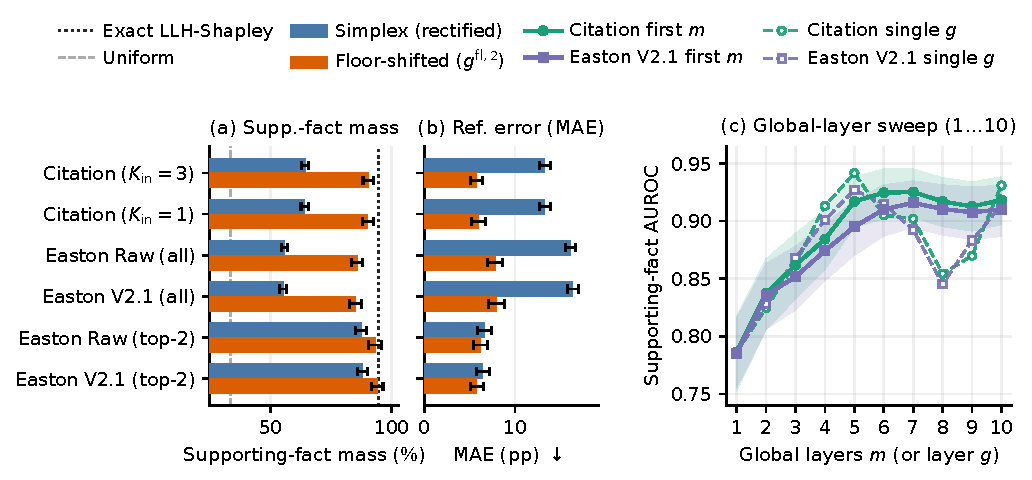
\includegraphics[width=0.98\linewidth]{figures/fig_citation_easton.pdf}
\caption{Direct attention heuristics on $200$ HotpotQA instances ($95\%$ bootstrap CIs). (a,~b)~Simplex (rectified) versus floor-shifted ($g^{\mathrm{fl},2}$) normalization on \texttt{mean10} for supporting-fact mass and MAE against exact LLH-Shapley. (c)~Supporting-fact AUROC across global-layer counts $m \in \{1, \dots, 10\}$ when averaging the first $m$ global layers (\texttt{first}~$m$, solid with $95\%$ CI bands) versus each individual global layer $\ell_g = 6g - 1$ (\texttt{single}~$g$, dashed).}
\label{fig:exp_citation_easton}
\end{figure}

\paragraph{Independent span scoring versus competitive per-step filtering.}
Both heuristics rank snippets accurately on HotpotQA (\texttt{mean10} AUROC $0.91$--$0.92$, P@2 $84.5$--$85.5\%$, Pearson $r = 0.91$--$0.92$), but they behave very differently under simplex normalization (Figure~\ref{fig:exp_citation_easton}(a,b)). Because Citation evaluates each snippet independently, entity-overlapping distractors always receive positive background attention, leaving $35.7\%$ ($42.5\%$ under \texttt{max10}) of the simplex mass on distractors and yielding $13.3$\,pp MAE. Applying $g^{\text{fl},2}$ removes this common floor without altering rankings, cutting Citation MAE from $13.3$ to $5.7$\,pp and lifting supporting-fact mass from $64.3\%$ to $90.6\%$. Conversely, Easton's competitive global \texttt{top-2} filter acts as an implicit hard floor: on $96.0\%$ of instances (\texttt{mean10}; $80.5\%$ under \texttt{max10}), at least one distractor receives exact zero weight ($\min_i s_i = 0$), so simplex normalization already achieves $6.4$\,pp MAE and $88.2\%$ supporting-fact mass ($5.8$\,pp and $94.3\%$ under $g^{\text{fl},2}$). Dropping the \texttt{top-2} filter (\emph{all tokens}) reintroduces background accumulation across distractor tokens, degrading supporting-fact mass to $55.3\%$ and AUROC to $0.88$.

\paragraph{Frequency penalty and head reduction.}
In Easton \texttt{top-2} (\texttt{mean10}), the most-attended snippet token is selected a median of $6$ times across the response; dampening repeats by $1/\sqrt{\operatorname{occ}_t(s)}$ in V2.1 consistently improves P@2 ($82.2\% \to 84.5\%$), AUROC ($0.90 \to 0.91$), Spearman $\rho$ ($0.76 \to 0.77$), and MAE ($6.6 \to 6.4$\,pp). Without per-step sparsification (\emph{all tokens}), however, every context token is included at every step so $\operatorname{occ}_t(s) = t$ merely reweights step $t$ by $t^{-1/2}$ rather than penalizing repeated token hits (whereas combining \emph{all tokens} with Stage-1 \texttt{max10+sp6} restores AUROC $0.90$ and $87.2\%$ mass). Across head reductions, averaging global heads and layers slightly outperforms elementwise maximization unless Stage-1 prefix pruning suppresses noisy outlier heads (\texttt{max10+sp24} lowers rectified Citation MAE from $15.8$ to $11.9$\,pp; \texttt{max10+sp6} raises Easton V2.1 Spearman $\rho$ to $0.78$).

\paragraph{How many global layers are worth aggregating?}
Sweeping every bottom-up prefix of $m \in \{1, \dots, 10\}$ global layers ($\ell \le 6m - 1$, matching early-exit serving budgets) reveals rapid initial gains followed by a sharp knee at half network depth (Figure~\ref{fig:exp_citation_easton}(c) and Table~\ref{tab:exp_citation_easton}). From $m = 1$ ($\ell = 5$) to $m = 5$ ($\ell \le 29$), supporting-fact AUROC climbs from $0.79$ to $0.92$ ($0.79 \to 0.84 \to 0.86 \to 0.88 \to 0.92$) for Citation and from $0.79$ to $0.90$ ($0.79 \to 0.84 \to 0.85 \to 0.87 \to 0.90$) for Easton V2.1, while MAE drops nearly in half ($11.3 \to 5.8$\,pp under $g^{\text{fl},2}$ for Citation; $12.5 \to 7.1$\,pp under simplex for Easton V2.1, as exact-zero distractor coverage rises from $58.0\%$ to $82.5\%$). By $m = 5$--$6$ ($50$--$60\%$ depth), prefix averaging already matches all $10$ global layers within $0.1$\,pp MAE, and it reaches a shallow optimum at $m = 6$--$7$ ($\ell \le 35$--$41$): at $m = 7$, Citation achieves AUROC $0.93$, P@2 $88.5\%$, $92.9\%$ mass, and $5.4$\,pp MAE, while Easton V2.1 reaches AUROC $0.92$, P@2 $86.5\%$, $89.0\%$ mass, and $6.0$\,pp MAE ($r = 0.92$, $\rho = 0.78$; elementwise maximization \texttt{max}$m$ and \texttt{max}$m$\texttt{+sp}$B$ saturate at the same $m = 6$--$7$ window). Including the remaining layers $m = 8$--$10$ brings no further improvement (P@2 softens slightly by $2$--$3$\,pp), so aggregating the first $6$--$7$ global layers---or $5$ under a tighter serving budget---captures the full accuracy while saving $30$--$50\%$ of global-layer extraction. Evaluating each global layer in isolation (\texttt{single}$g$, dashed curves in Figure~\ref{fig:exp_citation_easton}(c)) explains why: early layers $g = 1$--$3$ ($\ell \in \{5, 11, 17\}$) route a median $25.5$--$39.1\%$ of response attention to the BOS sink token (vs.\ $5.5$--$11.7\%$ in $g = 4$--$10$), single-layer accuracy peaks at the exact network midpoint $g = 5$ ($\ell = 29$; Citation AUROC $0.94$, P@2 $90.0\%$; Easton V2.1 AUROC $0.93$, P@2 $88.2\%$), dips in layers $g = 8$--$9$ ($\ell \in \{47, 53\}$, AUROC $0.85$--$0.88$), and rebounds at the final global layer $g = 10$ ($\ell = 59$, \texttt{last1}: Citation AUROC $0.93$, P@2 $88.0\%$, $5.8$\,pp MAE; Easton V2.1 AUROC $0.91$, P@2 $86.8\%$, $6.3$\,pp MAE). Contiguous bottom-up prefixes therefore require $m \ge 5$--$6$ layers to dilute early BOS-sink layers, whereas unrestricted layer selection can match or exceed $10$-layer averaging from a single mid-network or final global layer ($\ell = 29$ or $\ell = 59$).

\paragraph{Across benchmarks.}
Table~\ref{tab:exp_citation_easton_multi} evaluates the best-performing reductions on the other benchmarks with the same protocol and references as Table~\ref{tab:exp_multi}. The heuristics stay strong whenever the evidence is spread over distinct snippets: on 2WikiMultihopQA, Citation and Easton V2.1 reach AUROC $0.99$ and $r = 0.88$--$0.92$, and on CNN/DailyMail, where many sentences contribute to the summary, Easton V2.1 (\texttt{mean7}) reaches $r = 0.93$ and LDS $0.90$, more than any two-pass geometric method and close to ContextCite with $32$ ablations. On MuSiQue, Citation (\texttt{mean7}) reaches the highest supporting-fact AUROC of all methods ($0.94$, P@$k$ $80.7\%$) and Easton V2.1 $r = 0.94$, matching VATT with $v_{\text{logvol}}$. The duplicated-paragraph variant exposes limitation~(ii) below: the agreement of both heuristics with the reference drops to $r = 0.81$--$0.83$, and Easton V2.1 (\texttt{mean10}) gives one of the two copies less than $1\%$ of their joint credit in $19\%$ of the instances, because both copies compete for the same per-step top-$2$ tokens and the first match wins.

\begin{table}[t]
\centering
\small
\setlength{\tabcolsep}{3pt}
\resizebox{\linewidth}{!}{%
\begin{tabular}{llccccccccccccccc}
\toprule
 &  & \multicolumn{3}{c}{HotpotQA} & \multicolumn{3}{c}{2Wiki} & \multicolumn{3}{c}{MuSiQue} & \multicolumn{3}{c}{CNN/DM} & \multicolumn{3}{c}{Dup.} \\
\cmidrule(lr){3-5} \cmidrule(lr){6-8} \cmidrule(lr){9-11} \cmidrule(lr){12-14} \cmidrule(lr){15-17}
Heuristic & Link & $r$ & AUROC & MAE & $r$ & AUROC & MAE & $r$ & AUROC & MAE & $r$ & LDS & MAE & $r$ & AUROC & MAE \\
\midrule
Citation (\texttt{mean10}) & floor & 0.92 & 0.92 & 5.7 & 0.89 & 0.99 & 4.3 & 0.93 & 0.94 & 2.0 & 0.92 & 0.89 & 2.0 & 0.82 & 0.90 & 7.6 \\
Citation (\texttt{mean7}) & floor & 0.92 & 0.93 & 5.4 & 0.88 & 0.99 & 4.6 & 0.93 & 0.94 & 1.9 & 0.92 & 0.88 & 2.0 & 0.83 & 0.91 & 7.1 \\
Citation (\texttt{single5}) & floor & 0.89 & 0.94 & 6.2 & 0.85 & 0.99 & 5.0 & 0.90 & 0.94 & 2.5 & 0.87 & 0.85 & 2.6 & 0.83 & 0.93 & 6.6 \\
Easton V2.1 (\texttt{mean10}) & rect. & 0.92 & 0.91 & 6.4 & 0.91 & 0.99 & 3.9 & 0.94 & 0.92 & 1.8 & 0.93 & 0.89 & 1.8 & 0.81 & 0.88 & 8.2 \\
Easton V2.1 (\texttt{mean7}) & rect. & 0.92 & 0.92 & 6.0 & 0.92 & 0.99 & 3.8 & 0.94 & 0.93 & 1.8 & 0.93 & 0.89 & 1.8 & 0.82 & 0.89 & 7.9 \\
\midrule
VATT $v_{\mathrm{proj}}$ (for comparison) & floor & 0.91 & 0.93 & 5.8 & 0.88 & 0.99 & 4.6 & 0.91 & 0.90 & 2.9 & 0.85 & 0.85 & 2.9 & 0.84 & 0.91 & 6.7 \\
\bottomrule
\end{tabular}%
}
\caption{Direct attention heuristics across benchmarks (agreement with the reference of each benchmark; AUROC for supporting facts, LDS for CNN/DailyMail). VATT is repeated for comparison.}
\label{tab:exp_citation_easton_multi}
\end{table}

\paragraph{Structural limitations relative to cooperative-game attribution.}
Strong agreement on HotpotQA reflects its \emph{non-redundant} two-hop design: when two distinct paragraphs supply complementary facts, decoding attention aligns closely with ablation impact. Unlike cooperative-game values, however, raw attention heuristics lack three structural guarantees: (i)~\emph{uncalibrated context share}---context snippets absorb a median of only $43.5\%$ of \texttt{mean10} response attention (while the BOS sink token alone absorbs $15.8\%$) and unnormalized Citation totals depend strongly on the head reduction (median $\sum_i s_i^{\text{cit}} = 0.071$ on \texttt{mean10} vs.\ $1.88$ on \texttt{max10}), so separating parametric prior from context still requires the empty-context pass $w$; (ii)~\emph{no redundancy splitting}---scoring snippets independently gives two identical copies of a supporting paragraph the same raw score up to positional effects, so their combined simplex share is not split by a game but follows the attention pattern (split ratio $0.23$--$0.26$ on duplicated HotpotQA, vs.\ $0.39$ for the exact reference); and (iii)~\emph{routing versus counterfactual utility}---attention measures token lookup rather than causal entailment (e.g.\ attending to verify or negate a contradictory snippet, or favoring later positions under causal recency bias).